\section{Herleitung Kugeltransformation über Bandenreflektion}\label{anhang:herleitung:bandenreflektion}
Ein Zielpunkt $C$ wird an einer Bande gespiegelt, was im Punkt $\bar{C}$ resultiert. Gesucht wird der Punkt $A$ an
der Bande, welcher angespielt werden muss, damit der Zielpunkt $C$ getroffen wird. Dieser Punkt $A$ lässt sich über
den Schnittpunkt der Geraden, definiert durch die Bande, sowie der Geraden zwischen dem Punkt $\bar{C}$ und dem Punkt
$B$ bestimmen. Anzumerken sei hier, dass im Falle einer zweidimensionalen Betrachtung die Bande um den Radius in Richtung
Zentrum verschoben werden muss, um den korrekten Anspielpunkt $A$ zu finden.

Es ergeben sich dadurch die beiden Linien:
\begin{align}
    \vec{l} &= \vec{\bar{C}} - \vec{B}\\
    L_1 &= \vec{B} + \lambda_1 \cdot \vec{l}\\
    \vec{r} &= \vec{R_2} - \vec{R_1}\\
    L_2 &= \vec{R_1} + \lambda_2 \cdot \vec{r}
\end{align}
Der Schnittpunkt kann über die in Kapitel \ref{anhang:herleitung:linie-linie-schnittpunkt} vorgestellte Formel
berechnet werden.
\begin{align}
    \lambda_1 = \frac{r_x \cdot B_y - r_y \cdot B_x + R_{1,x} \cdot r_y - R_{1,y} \cdot r_x}{l_x \cdot r_y - \cdot l_y \cdot r_x}
\end{align}

\subsection{Den gespiegelten Zielpunkt bestimmen}\label{anhang:herleitung:bandenreflektion:zielpunkt}
Um den gespiegelten Zielpunkt $\bar{C}$ zu bestimmen, wird in einem ersten Schritt das Koordinatensystem transformiert, damit
der Ursprung bei einem der Eckpunkte an der zu spiegelnden Bande liegt. Sind die Start- und Endpunkte $R^1$ sowie $R^2$
gegeben und der Ursprung soll zum Startpunkt $R^1$ verschoben werden, kann die folgende Transformationsmatrix in
homogenen Koordinaten angewendet werden:
\begin{align}
    T^0 = \begin{pmatrix}1 & 0 & -R^1_x\\0 & 1 & -R^1_y\\0 & 0 & 1\end{pmatrix}
\end{align}
Die Transformation für einen Punkt $C$ in homogenen Koordinaten lautet demnach:
\begin{align}
    C_0 = T^0 \cdot C
\end{align}

In einem weiteren Schritt kann der transformierte Zielpunkt $C$ gespiegelt werden. Diese Spiegelung geschieht durch
Multiplikation mit einem Vektor $\vec{s}$. Für die Herleitung kann Abbildung \ref{fig:bandenspiegelung} hinzugezogen werden.

\begin{figure}[h!]
    \begin{center}
        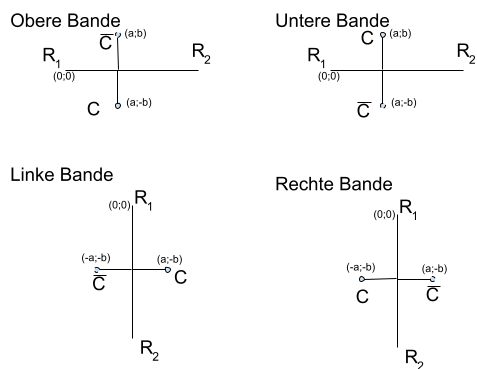
\includegraphics[width=0.8\linewidth]{../common/07_appendix/resources/02_bandenspiegelung.png}
    \end{center}
    \caption{Spiegelung an den verschiedenen Banden}
    \label{fig:bandenspiegelung}
\end{figure}

Aus dieser Abbildung ergeben sich die nachfolgenden Beziehungen:
\begin{align}
    \begin{pmatrix}a \\ -b\end{pmatrix} &\rightarrow \begin{pmatrix}a \\ b\end{pmatrix}\\
    \begin{pmatrix}a \\ b\end{pmatrix} &\rightarrow \begin{pmatrix}a \\ -b\end{pmatrix}\\
    \begin{pmatrix}a \\ -b\end{pmatrix} &\rightarrow \begin{pmatrix}-a \\ -b\end{pmatrix}\\
    \begin{pmatrix}-a \\ -b\end{pmatrix} &\rightarrow \begin{pmatrix}a \\ -b\end{pmatrix}\\
\end{align}

Anhand der Beziehungen kann für die obere sowie untere Bande folgende Eigenschaft gefunden werden:
\begin{align}
    \vec{\bar{C}} = \vec{C} \cdot \begin{pmatrix}1 \\ -1\end{pmatrix}
\end{align}
Für die linke sowie rechte Bande lautet die Eigenschaft:
\begin{align}
    \vec{\bar{C}} = \vec{C} \cdot \begin{pmatrix}-1 \\ 1\end{pmatrix}
\end{align}

Um den korrekten Vektor $\vec{s}$ für die Spiegelung zu wählen, kann eine Funktion über die Normale auf die jeweilige Bande
angewendet werden (es wird angenommen, dass die Banden horizontal oder vertikal verlaufen, ansonsten müsste zuerst eine
entsprechende Rotation ergänzt werden). Es ergeben sich folgende Beziehungen für die obere und untere Bande. Zu beachten ist, dass $R^1$ und $R^2$ bei den
jeweiligen Bandensegmenten auch vertauscht werden
können, weswegen die Normalen auch in die entgegengesetzte Richtung zeigen können. Aus diesem Grund werden beide Fälle
betrachtet.
\begin{align}
    \begin{pmatrix}0 \\ -1\end{pmatrix} \xrightarrow{f} \begin{pmatrix}1 \\ -1\end{pmatrix}\\
    \begin{pmatrix}0 \\ 1\end{pmatrix} \xrightarrow{f} \begin{pmatrix}1 \\ -1\end{pmatrix}\\
\end{align}
Dasselbe gilt für die linke und rechte Bande:
\begin{align}
    \begin{pmatrix}1 \\ 0\end{pmatrix} \xrightarrow{f} \begin{pmatrix}-1 \\ 1\end{pmatrix}\\
    \begin{pmatrix}-1 \\ 0\end{pmatrix} \xrightarrow{f} \begin{pmatrix}-1 \\ 1\end{pmatrix}\\
\end{align}

Da die Abbildungen nicht injektiv, aber surjektiv sind, kann jeweils nur der Absolutwert der Normalen betrachtet
werden. Die Beziehungen reduzieren sich auf zwei:
\begin{align}
    \begin{pmatrix}0 \\ 1\end{pmatrix} \xrightarrow{f} \begin{pmatrix}1 \\ -1\end{pmatrix}\\
    \begin{pmatrix}1 \\ 0\end{pmatrix} \xrightarrow{f} \begin{pmatrix}-1 \\ 1\end{pmatrix}\\
\end{align}
Es wird eine lineare Funktion gesucht, welche die Abbildung darstellt:
\begin{align}
    f(\vec{x}) &= a \cdot \vec{x} + \vec{b}\\
    \begin{pmatrix}1 \\ -1\end{pmatrix} &= a \cdot \begin{pmatrix}0 \\ 1\end{pmatrix} + \begin{pmatrix}b_x \\ b_y\end{pmatrix}\\
    \begin{pmatrix}-1 \\ 1\end{pmatrix} &= a \cdot \begin{pmatrix}1 \\ 0\end{pmatrix} + \begin{pmatrix}b_x \\ b_y\end{pmatrix}
\end{align}

Daraus ergeben sich vier Gleichungen:
\begin{align}
    1 &= b_x\\
    -1 &= a + b_y\\
    -1 &= a + b_x\\
    1 &= b_y
\end{align}
Demnach lauten die Parameter:
\begin{align}
    b_x &= 1\\
    b_y &= 1\\
    a &= -2
\end{align}
Anhand der nachfolgenden Funktion kann der Spiegelvektor $\vec{s}$ bestimmt werden:
\begin{align}
    \vec{s} = \hat{n} \cdot -2 + \vec{1}
\end{align}

Die Spiegelung kann ebenfalls als Transformation $S$ in homogenen Koordinaten ausgedrückt werden:
\begin{align}
    S = \begin{pmatrix}s_x & 0 & 0 \\ 0 & s_y & 0 \\ 0 & 0 & 1\end{pmatrix}
\end{align}

Abschliessend wird die erhaltene Position in das ursprüngliche Koordinatensystem überführt:
\begin{align}
    T = \begin{pmatrix}1 & 0 & R^1_x\\0 & 1 & R^1_y\\0 & 0 & 1\end{pmatrix}
\end{align}

Die gesamte Transformation kann über die Matrix $M$ ausgedrückt werden:
\begin{align}
    M = T \cdot S \cdot T^0\\
    M = \begin{pmatrix}s_x & 0 & R^1_x - s_x \cdot R^1_x \\ 0 & s_y & R^1_y - s_y \cdot R^1_y \\ 0 & 0 & 1\end{pmatrix}
\end{align}

Demnach wird der gespiegelte Punkt $\bar{C}$ wie folgt bestimmt, wobei die zusätzliche Z-Komponente weggelassen werden
kann:
\begin{align}
    \bar{C} = M \cdot C
\end{align}